\documentclass[a4paper]{article}
\usepackage{array}  
\usepackage[table]{xcolor}% http://ctan.org/pkg/xcolor
\usepackage{geometry}
\geometry{margin=1.25in}
\usepackage{hhline}
\usepackage{environ}
\usepackage{graphicx}
 %\geometry{
 %a4paper,z
 %total={170mm,257mm},
 %left=40mm,
 %right=40mm
 %}
 \newcommand{\colWidth}{141mm}

\begin{document} 
\section*{Demo day: \textit{(demo 2)} Group \textit{(group 10)}}

% ------------GOALS----------

\begin{center}
\begin{tabular}{|p{\colWidth}|}
	\hline
	\cellcolor{blue!25}\large
	\textbf{What were your goals?}
	\\ \hline
	\vtop to 130mm{
\begin{itemize}
    \item B.O.B Hardware
    \begin{itemize}
         \item Build B.O.B prototype grabber. 
         \item Build arena/shop construction. 
         \item Stretch goal: Build and test the lifting mechanism.
         \item Stretch goal: Build B.O.B prototype basket.
    \end{itemize}
    \item B.O.B Software
    \begin{itemize} 
        \item Reverse/Backwards movement.
        \item Implement B.O.B taking orders from server. Follows path given by server; takes items to bagging station.
        \item Stretch goal: Correct direction of travel when not on line.
        \item Stretch goal: Sideways movement across multiple aisles. 
    \end{itemize}
    \item Server: 
    \begin{itemize}
        \item Database fully implemented (includes updating and maintenance). 
        \item Implement Path-finding for B.O.B.
    \end{itemize}
    \item App:
    \begin{itemize}
        \item Main functionality present (Customer Login/Registration, Viewing Warehouses and items, Placing Orders).
        \item Adopt new features on the Server.
        \item More realistic User Interface.
    \end{itemize}
    \item Website: 
    \begin{itemize}
        \item Managing of Warehouses and Items functionality.
        \item Creating Front-end authentication of website. 
        \item Defining Website structure.
        \item B.O.B has Logo.
    \end{itemize}
\end{itemize}
  }
  \\
  %have database - connects - get order and stuff - FOR SERVER
  \hline
\end{tabular}
\vskip 5mm

% ------------ORGANISATION----------

\begin{tabular}{|p{\colWidth}|}
	\hline
	\cellcolor{blue!25}\large
	\textbf{Summarise how your group organised the workload to achieve your goals.}
	\\ \hline
	\vtop to 80mm{
	\begin{itemize}
	    \item Team Split
	    \begin{itemize}
	        \item Robot Hardware
	        \item Robot Software
	        \item Server, Website and App 
	    \end{itemize}
	    \item Robot Hardware
	    \begin{itemize}
	        \item Jacob, Anna built B.O.B's arena.
	        \item Anna built B.O.B's claw and basket.
	        \item Jacob built lift mechanism.
	    \end{itemize}
	    \item Robot Software
	    \begin{itemize}
	        \item Claire and Alex worked on B.O.B movement. Anna assisted. 
	    \end{itemize}
	    \item Server, Website and App 
	    \begin{itemize}
	        \item Freddie, Kieran and Oktay improved the server.
	        \item Oktay improved the App.
	        \item Harry improved the Website.
	    \end{itemize}
	\end{itemize}
  }
  \\
  \hline
\end{tabular}
\vskip 5mm

% ------------ACHIEVEMENTS----------

\begin{tabular}{|p{\colWidth}|}
	\hline
	\cellcolor{blue!25}\large
	\textbf{What were your main achievements?}
	\\ \hline
	\vtop to 30mm{
	\begin{itemize}
	    \item Customers can view warehouses and items, and place orders via App with a user-friendly interface.
	    \item Stretch goal: B.O.B lifting mechanism built and tested.
	    \item B.O.B takes orders from server (follows path to take items to bagging station).
	    \item Stretch goals: B.O.B can correct direction of travel when not on line. Sideways movement across multiple aisles.
	\end{itemize}
  }
  \\
  \hline
\end{tabular}
\vskip 5mm

% ------------NOT ACHIEVED----------

\begin{tabular}{|p{\colWidth}|}
	\hline
	\cellcolor{blue!25}\large
	\textbf{What did you not achieve? Briefly explain why.}
	\\ \hline
	\vtop to 10mm{
	\begin{itemize}
	    \item User QR code not generated. Prioritised lifting mechanism due to concerns addressed in first demo by the experts.
	\end{itemize}
  }
  \\
  \hline
\end{tabular}
\vskip 5mm

% ------------NEXT STEPS----------

\begin{tabular}{|p{\colWidth}|}
	\hline
	\cellcolor{blue!25}\large
	\textbf{Say briefly what changes you will make to your plan for the next demo.}
	\\ \hline
	\vtop to 20mm{
	\begin{itemize}
	    \item User QR Code Generation.
	    \item Construct shelves.
	    \item Stabilise/Improve B.O.B sideways movement.
	\end{itemize}
  }
  \\
  \hline
\end{tabular}

% ------------QUANTITIVE----------
\newpage
\begin{tabular}{|p{\colWidth}|}
	\hline
	\cellcolor{blue!25}\large
	\textbf{Include any quantitative data you have collected (this can be a graph/table with a few words)}
  \\
  \hline
\end{tabular}

\begin{figure}[!htb]
\minipage{0.45\textwidth}
  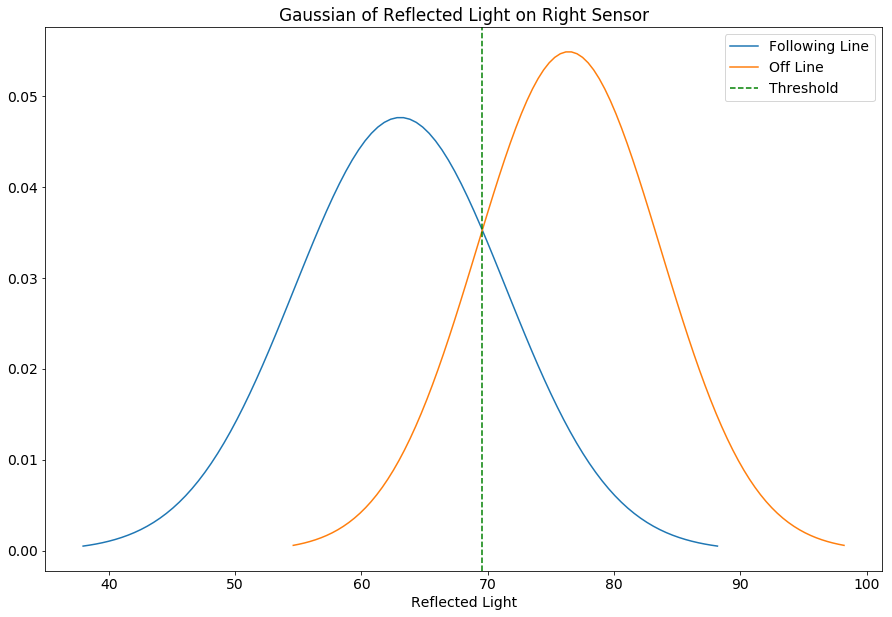
\includegraphics[width=\linewidth]{stay_on_line.png}
  \caption{Difference of sensor readings with regards to motor speed.}\label{fig:awesome_image1}
\endminipage\hfill
    \minipage{0.55\textwidth}
     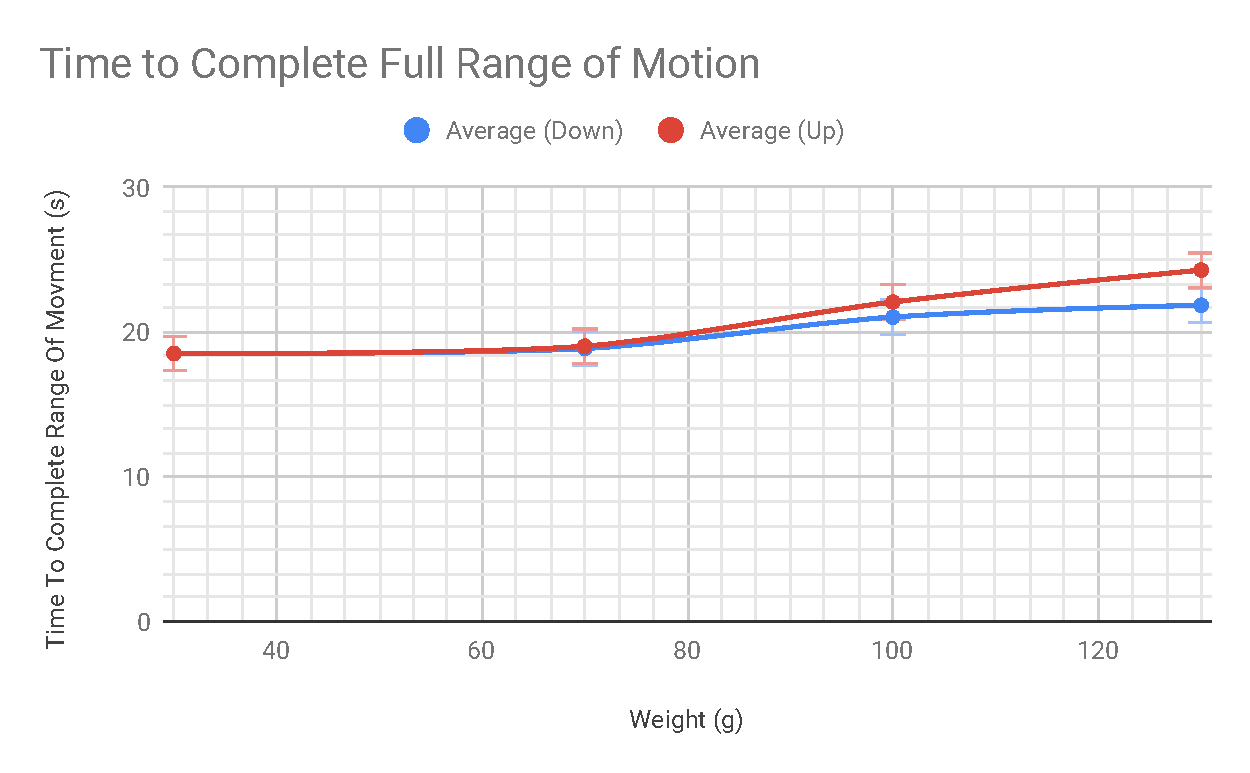
\includegraphics[width=\textwidth]{time_range_of_motion.pdf}
     \caption{Affect of varied weights when covering 1 meter}\label{fig:awesome_image2}
\endminipage
\newline
\end{figure}

\begin{table}[!htb]
\centering
\begin{tabular}{| p{2cm} | p{2cm} | p{2cm} | p{2cm} |}
\hline
\textbf{Item} & \textbf{Cost Per Unit} & \textbf{Quantity} & \textbf{Total Cost} \\
\hline
EV3 Colour Sensor & £30.00 & 2 & £60.00 \\
\hline
Omni Wheels & £6.60 & 6 & £39.60 \\
\hline
MDF Panels & £6.00 & 6 & £36.00 \\
\hline
Hypothetical Server Cost & £15.00 & 1 & £15.00 \\ 
\hline
 &  & \textbf{Total} & £150.60 \\ 
\hline
 &  & \textbf{Balance} & £49.40 \\
\hline
\end{tabular}
\caption{Finance}
\end{table}


\begin{table}[!htb]
\centering
\begin{tabular}{| p{2cm} | p{2cm} |}
\hline
\textbf{Battery (mAh)} & \textbf{Voltage} \\
\hline
2200 & 7.5V \\
\hline
\end{tabular}
\caption{EV3 Battery and Voltage}
\end{table}

\begin{table}[!htb]
\centering
\begin{tabular}{| p{2.2cm} | p{2cm} | p{2.2cm} | p{2cm} | p{2cm} |}
\hline
\textbf{Component} & \textbf{Amperes (7.5V)} & \textbf{Number on Board} & \textbf{Total Amperes} & \textbf{Total mA}\\
\hline
Colour Sensor & 0.107 & 4 & 0.428 & 428 \\
\hline
Motor (Running at 100\%) & 0.186 & 5 & 0.930 & 930 \\
\hline 
Processor (Running at 100\%) & 0.098 & 1 & 0.098 & 98 \\
\hline
 & & & \textbf{Battery Time From Full Charge (Hours)} & 1.511 \\ 
 \hline
\end{tabular}
\caption{Source https://www.dexterindustries.com/ev3-current-consumption-measurement/}
\end{table}

\begin{table}[!htb]
\centering
\begin{tabular}{| p{2cm} | p{2cm} | p{2cm} | p{2cm} | p{2cm} |}
\hline
\textbf{Weight (g)} & \textbf{Time (s)-Run 1} & \textbf{Time (s)-Run 2} & \textbf{Time (s)-Run 3} & \textbf{Time (s)-Run 4} \\
\hline
0 & 0.107 & 0 & 0 & 0 \\
\hline
50 & 0.186 & 0 & 0 & 0 \\
\hline 
80 & 0.098 & 0 & 0 & 0 \\
 \hline
\end{tabular}
\caption{Source https://www.dexterindustries.com/ev3-current-consumption-measurement/}
\end{table}

\begin{figure}[!htb]
  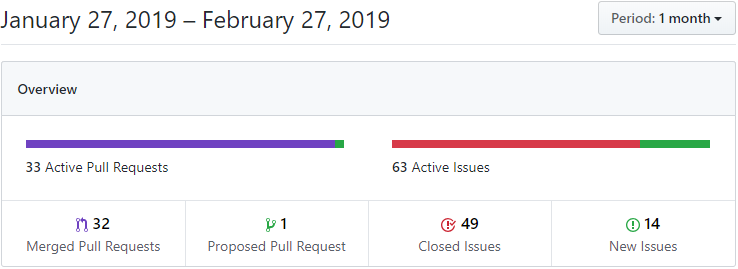
\includegraphics[width=\linewidth]{github-contributions.PNG}
  \caption{GitHub contributions during the month before Demo 2. 63 issues were worked on, out of which 49 were closed. Of the 49 closed issues, 32 resulted in changes to code that were approved and merged.}\label{fig:awesome_image3}
\end{figure}

\end{center}
  
\end{document}
